%%%%%%%% ICML 2022 EXAMPLE LATEX SUBMISSION FILE %%%%%%%%%%%%%%%%%

\documentclass[nohyperref]{article}

% Recommended, but optional, packages for figures and better typesetting:
\usepackage{microtype}
\usepackage{graphicx}
\usepackage{subfigure}
\usepackage{booktabs} % for professional tables

% hyperref makes hyperlinks in the resulting PDF.
% If your build breaks (sometimes temporarily if a hyperlink spans a page)
% please comment out the following usepackage line and replace
% \usepackage{icml2022} with \usepackage[nohyperref]{icml2022} above.
\usepackage{hyperref}


% Attempt to make hyperref and algorithmic work together better:
\newcommand{\theHalgorithm}{\arabic{algorithm}}

% Use the following line for the initial blind version submitted for review:
%\usepackage{icml2022}

% If accepted, instead use the following line for the camera-ready submission:
\usepackage[accepted]{icml2022}

% For theorems and such
\usepackage{amsmath}
\usepackage{amssymb}
\usepackage{mathtools}
\usepackage{amsthm}

% if you use cleveref..
\usepackage[capitalize,noabbrev]{cleveref}

%%%%%%%%%%%%%%%%%%%%%%%%%%%%%%%%
% THEOREMS
%%%%%%%%%%%%%%%%%%%%%%%%%%%%%%%%
\theoremstyle{plain}
\newtheorem{theorem}{Theorem}[section]
\newtheorem{proposition}[theorem]{Proposition}
\newtheorem{lemma}[theorem]{Lemma}
\newtheorem{corollary}[theorem]{Corollary}
\theoremstyle{definition}
\newtheorem{definition}[theorem]{Definition}
\newtheorem{assumption}[theorem]{Assumption}
\theoremstyle{remark}
\newtheorem{remark}[theorem]{Remark}

% Todonotes is useful during development; simply uncomment the next line
%    and comment out the line below the next line to turn off comments
%\usepackage[disable,textsize=tiny]{todonotes}
\usepackage[textsize=tiny]{todonotes}


% The \icmltitle you define below is probably too long as a header.
% Therefore, a short form for the running title is supplied here:
\icmltitlerunning{Extremum Seeking Gradient}

\begin{document}

\twocolumn[
\icmltitle{Extremum Seeking Gradient \\ Machine Learning without Backpropagation}

% It is OKAY to include author information, even for blind
% submissions: the style file will automatically remove it for you
% unless you've provided the [accepted] option to the icml2022
% package.

% List of affiliations: The first argument should be a (short)
% identifier you will use later to specify author affiliations
% Academic affiliations should list Department, University, City, Region, Country
% Industry affiliations should list Company, City, Region, Country

% You can specify symbols, otherwise they are numbered in order.
% Ideally, you should not use this facility. Affiliations will be numbered
% in order of appearance and this is the preferred way.
\icmlsetsymbol{equal}{*}

\begin{icmlauthorlist}
\icmlauthor{Or Dicker}{yyy}
\icmlauthor{David Prichen}{yyy}
%\icmlauthor{Firstname3 Lastname3}{comp}
%\icmlauthor{Firstname4 Lastname4}{sch}
%\icmlauthor{Firstname5 Lastname5}{yyy}
%\icmlauthor{Firstname6 Lastname6}{sch,yyy,comp}
%\icmlauthor{Firstname7 Lastname7}{comp}
%\icmlauthor{}{sch}
%\icmlauthor{Firstname8 Lastname8}{sch}
%\icmlauthor{Firstname8 Lastname8}{yyy,comp}
%\icmlauthor{}{sch}
%\icmlauthor{}{sch}
\end{icmlauthorlist}

\icmlaffiliation{yyy}{Department of Electrical Engineering, Tel Aviv University}
%\icmlaffiliation{comp}{Company Name, Location, Country}
%\icmlaffiliation{sch}{School of ZZZ, Institute of WWW, Location, Country}

\icmlcorrespondingauthor{Or Dicker}{or.dicker@gmail.co.il}
\icmlcorrespondingauthor{David Prichen}{first2.last2@gmail.co.il}

% You may provide any keywords that you
% find helpful for describing your paper; these are used to populate
% the "keywords" metadata in the PDF but will not be shown in the document
\icmlkeywords{Machine Learning, ICML, Extremum Seeking}

\vskip 0.3in
]

% this must go after the closing bracket ] following \twocolumn[ ...

% This command actually creates the footnote in the first column
% listing the affiliations and the copyright notice.
% The command takes one argument, which is text to display at the start of the footnote.
% The \icmlEqualContribution command is standard text for equal contribution.
% Remove it (just {}) if you do not need this facility.

\printAffiliationsAndNotice{}  % leave blank if no need to mention equal contribution
%\printAffiliationsAndNotice{\icmlEqualContribution} % otherwise use the standard text.

\begin{abstract}
This document provides a basic paper template and submission guidelines.
Abstracts must be a single paragraph, ideally between 4--6 sentences long.
Gross violations will trigger corrections at the camera-ready phase.
\end{abstract}

\section{Introduction}
\subsection{Analog Neural Network}

Photonic Neural Network \cite{Pai_2023}
\subsection{What is wrong with backpropagation}
Hinton claims that propagation can't be how the brain learns as a model e despite considerable effort to
invent ways in which it could be implemented by real neurons. There is no convincing evidence
that cortex explicitly propagates error derivatives or stores neural activities for use in a subsequent
backward pass. The top-down connections from one cortical area to an area that is earlier in the
visual pathway do not mirror the bottom-up connections as would be expected if backpropagation
was being used in the visual system. Instead, they form loops in which neural activity goes through
about half a dozen cortical layers in the two areas before arriving back where it started.
Backpropagation through time as a way of learning sequences is especially implausible. To deal with
the stream of sensory input without taking frequent time-outs, the brain needs to pipeline sensory
data through different stages of sensory processing and it needs a learning procedure that can learn
on the fly. The representations in later stages of the pipeline may provide top-down information
that influences the representations in earlier stages of the pipeline at a later time step, but the
perceptual system needs to perform inference and learning in real time without stopping to perform
backpropagation.A further serious limitation of backpropagation is that it requires perfect knowledge of the computation
performed in the forward pass in order to compute the correct derivatives If we insert a black
box into the forward pass, it is no longer possible to perform backpropagation unless we learn a
differentiable model of the black box.
We believe that ESG learning algorithm \cref{alg:ESG-analog} could overcame these limitation and, but different hardware is needed to compete with backpropagation performance.   

\subsection{Extremum Seeking Control}
Extremum seeking control is a dynamic optimization technique employed in control systems to seek and maintain the optimal operating point of a system, often in the presence of changing or uncertain conditions. It operates by systematically perturbing a control input and observing the resulting system response to detect changes in a chosen performance metric. By continuously adjusting the control input in the direction that improves or maximizes the observed metric, extremum seeking control can adapt to variations in the system and ensure optimal performance. This approach is particularly valuable in applications where precise modeling of system dynamics is challenging, offering a versatile and robust solution for optimizing processes and systems in real-time.

\begin{figure}[ht]
\vskip 0.2in
\begin{center}
\centerline{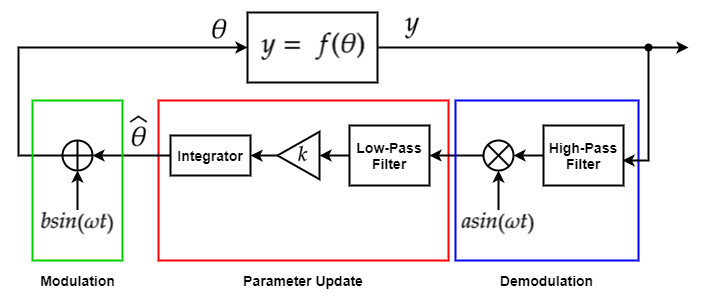
\includegraphics[width=\columnwidth]{images/esc_static_optimization.png}}
\caption{}
\end{center}
\vskip -0.2in
\end{figure}

\begin{figure}[ht]
\vskip 0.2in
\begin{center}
\centerline{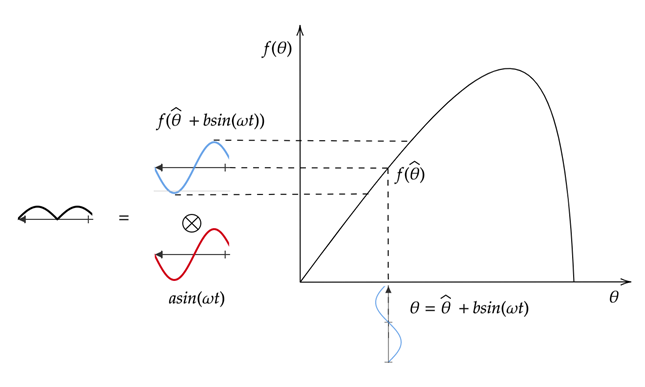
\includegraphics[width=\columnwidth]{images/esc_increasing_objective.png}}
\caption{}
\end{center}
\vskip -0.2in
\end{figure}


\section{Algorithm}
\begin{figure*}[ht]
\vskip 0.2in
\begin{center}
\centerline{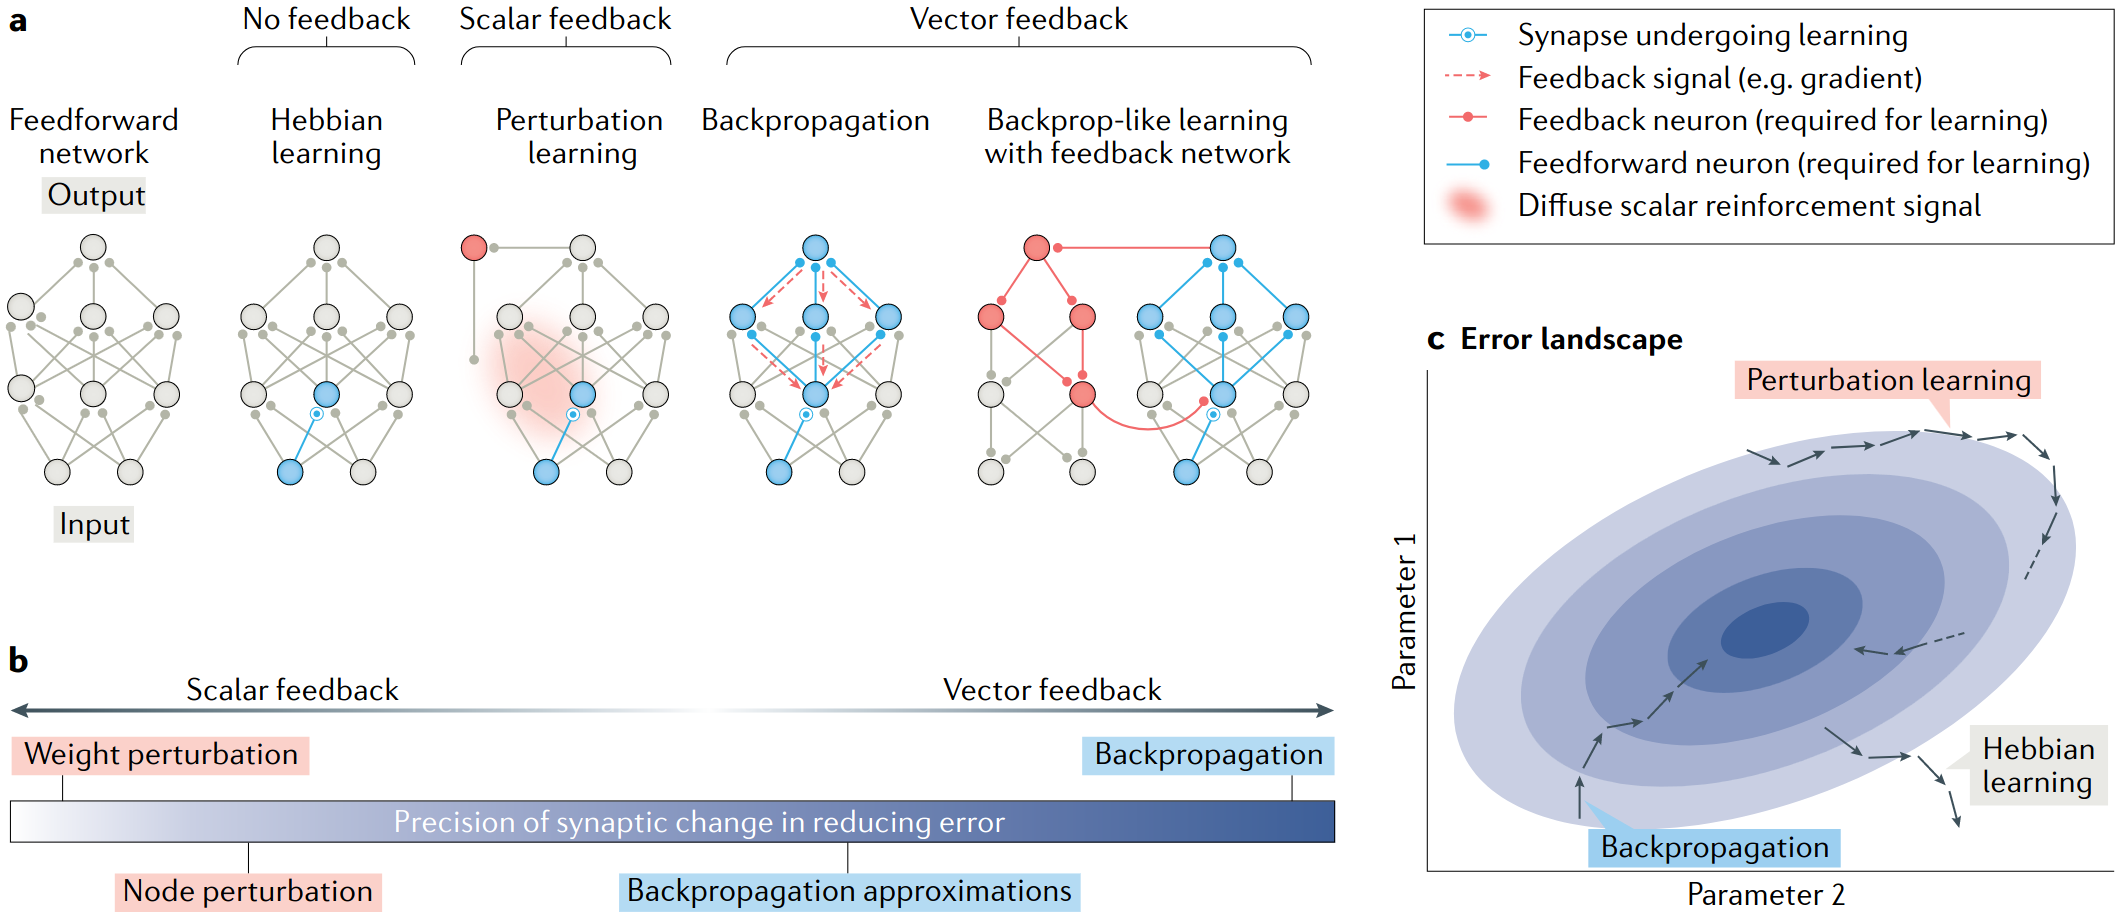
\includegraphics[width=2\columnwidth]{images/grad_landscape.png}}
\caption{\textbf{A spectrum of learning algorithms}| From left to right, a neural network processes data through simple computational units and adjusts the connections (synapses) between these units to enhance its performance on a given task. Traditional Hebbian learning, which strengthens synapses when a presynaptic neuron consistently contributes to a postsynaptic neuron's firing, cannot effectively modify certain synapses because it doesn't account for their downstream impact on the network's overall output.}
\label{grad_landscape}
\end{center}
\vskip -0.2in
\end{figure*}

\subsection{Backpropagation}
Backpropagation\cref{alg:BP}, a fundamental algorithm in the field of deep learning, offers substantial advantages in terms of computational efficiency, especially when dealing with inputs of significantly larger dimensions than the network's initial layer. This characteristic becomes particularly relevant in today's era of big data and complex information processing tasks.

One of the primary advantages of backpropagation in such scenarios is its ability to efficiently calculate gradients for each layer of a deep neural network. When the input dimensionality is high, traditional optimization techniques become computationally prohibitive due to the curse of dimensionality. However, backpropagation mitigates this challenge by propagating errors backward through the layers, effectively distributing the computation of gradients across the network. This distributed computation not only reduces the computational burden but also allows for parallelization, which can be leveraged with modern hardware, such as GPUs and TPUs, to expedite the training process.

\begin{algorithm}[tb]
     \caption{Backpropagation}
   \label{alg:BP}

  \begin{algorithmic}
\STATE Compute the error at the output layer:
\STATE $\delta^{(L)} = \nabla_a \mathcal{L} \odot \sigma'(z^{(L)})$
\FOR{each layer $l$ from $L-1$ to $1$}
    \STATE Backpropagate the error through the layers:
    \STATE $\delta^{(l)} = ((W^{(l+1})^T \delta^{(l+1)}) \odot \sigma'(z^{(l)})$
    \STATE Calculate the gradients of the weights and biases:
    \STATE $\nabla W^{(l)} = \delta^{(l)}(a^{(l-1)})^T$
    \STATE $\nabla b^{(l)} = \delta^{(l)}$
\ENDFOR    
\end{algorithmic}
\end{algorithm}



\subsection{Forward Forward Algorithm(Hebbian Learning)}
Hebbian learning is a fundamental concept in neuroscience and artificial neural networks, describing a synaptic plasticity rule that governs how the strength of connections between neurons evolves over time. Named after the psychologist Donald Hebb, it is often summarized by the phrase "cells that fire together, wire together." In essence, if two neurons are frequently active at the same time, the synaptic connection between them is strengthened. This process reinforces the association between neurons and is believed to play a critical role in learning and memory formation. Hebbian learning has also influenced the development of artificial neural networks, where it has been used as a foundational principle for training models to capture patterns and relationships in data.

The Forward-Forward algorithm\cite{hinton2022forward}, introduced by Geoffrey Hinton, represents a novel and innovative approach to deep learning that draws inspiration from Boltzmann machines and Noise Contrastive Estimation. Unlike traditional backpropagation, this method employs two forward passes that operate symmetrically but on distinct datasets with opposing objectives. The positive pass refines network weights to enhance representations for real data, while the negative pass adjusts weights to diminish quality for negative data. This unique framework allows for the exploration of various quality metrics. The ultimate aim of the Forward-Forward algorithm is to effectively classify input vectors as positive or negative data based on a logistic function applied to the quality metric, making it a promising and versatile addition to the arsenal of deep learning techniques.

Let us suppose that the goodness function for a layer is simply the sum of the squares of the activities
of the rectified linear neurons in that layer4 The aim of the learning is to make the goodness be
well above some threshold value for real data and well below that value for negative data. More
specifically, the aim is to correctly classify input vectors as positive data or negative data when the probability that an input vector is positive (i. e. real) is given by applying the logistic function, $\sigma$ to the goodness, minus some threshold $\theta$
$$p(positive) = \sigma(\sum_{j}y^{2}_{j}-\theta)$$
where $y_{j}$ is the activity of hidden unit $j$ before layer normalization. 

\begin{figure}[ht]
\vskip 0.2in
\begin{center}
\centerline{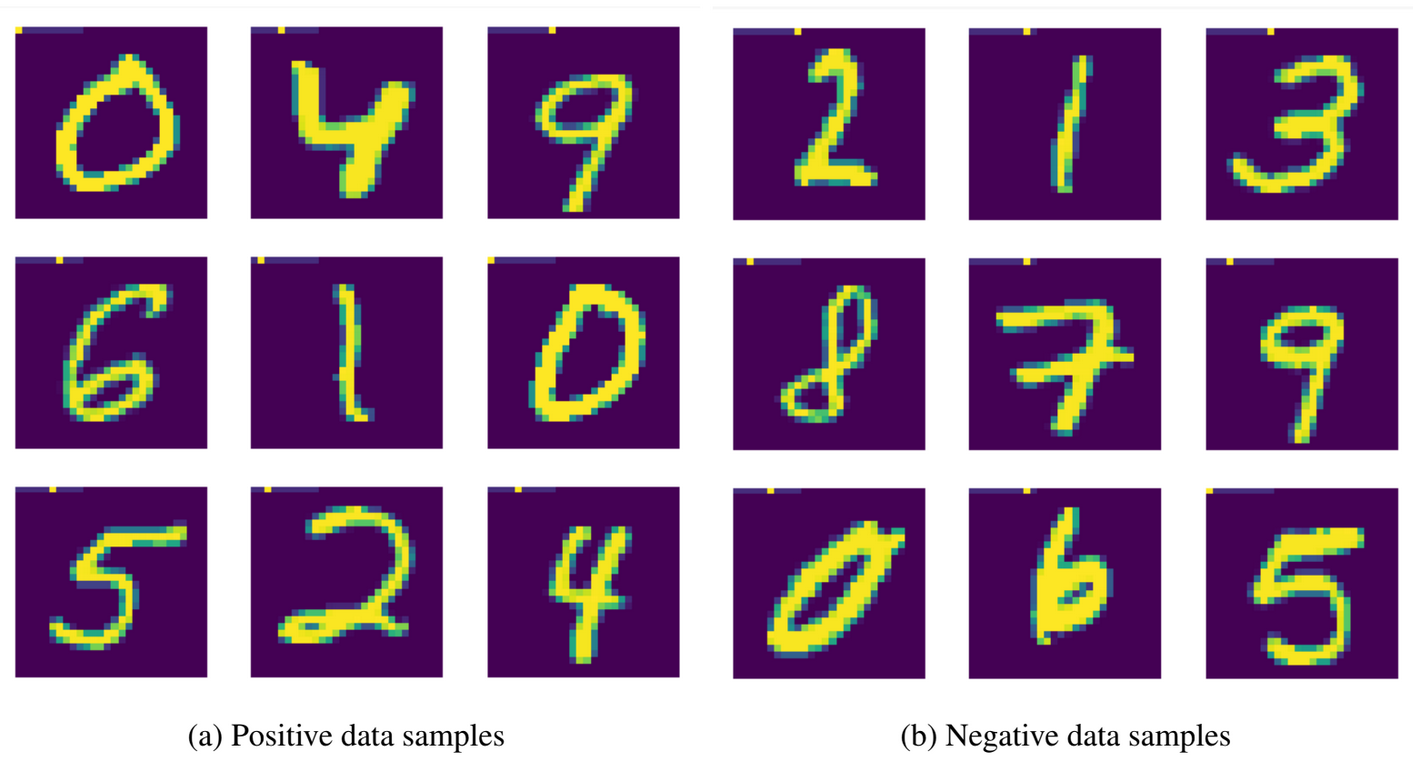
\includegraphics[width=\columnwidth]{images/FF_embedding.png}}
\caption{Data embedding for Forward Forward algorithm. The label can be seen in the top left 10 pixels}
  \label{fig:FF_embed}
\end{center}
\vskip -0.2in
\end{figure}


\begin{algorithm}[tb]
   \caption{Forward Forward}
   \label{alg:FF}
\begin{algorithmic}
   \STATE {\bfseries Input:} dataset $\{x_{i},y_{i}\}$, NN architecture $f(x;\theta)$, NN parameters $\theta$, goodness $\theta(\hat{y},y)$ 
   \FOR{each training example $(x^{(i)}, y^{(i)})$}
   \STATE \textbf{Positive Pass:}
   \STATE embed $(x^{(i)}, y^{(i)})$ together like fig \ref{fig:FF_embed}
    \STATE Perform a forward pass with real data to compute the goodness metric.
    \STATE Adjust the weights to increase the goodness above a threshold for real data.
    \STATE \textbf{Negative Pass:}
    \STATE embed $(x^{(i)}, \tilde{y}^{(i)})$  where $\tilde{y}$ is random
    \STATE Perform a forward pass with "negative data" to compute the goodness metric.
    \STATE Adjust the weights to decrease the goodness below the threshold for negative data.
\ENDFOR
\end{algorithmic}
\end{algorithm}

\subsubsection{multaneous-perturbation stochastic
approximation (SPSA) (gradient part)}
Simultaneous Perturbation Stochastic Approximation (SPSA)\cref{alg:SPSA} is a powerful optimization technique used primarily in scenarios where obtaining precise gradient information for a complex objective function is challenging or computationally expensive. SPSA is particularly valuable in the field of optimization and has found applications in various domains, including engineering, machine learning, and operations research.

At its core, SPSA is a gradient-free optimization method designed to efficiently search for the optimal solution within a parameter space, typically characterized by a high dimensionality. This technique is particularly well-suited for scenarios where the underlying objective function is non-convex, noisy, or lacks a readily available closed-form expression.

The distinguishing feature of SPSA is its use of simultaneous perturbations, where it estimates the gradient of the objective function by evaluating the function at two different points, perturbed in opposite directions along each parameter axis. By analyzing the difference in function values resulting from these perturbations, SPSA approximates the gradient direction, allowing it to iteratively update the parameter values towards the optimum.

\begin{algorithm}[tb]
   \caption{SPSA}
   \label{alg:SPSA}
\begin{algorithmic}
  \STATE {\bfseries Input:} dataset $\{x_{i},y_{i}\}$, NN architecture $f(x;\theta)$, NN parameters $\theta$, Loss function $L(\hat{y},y)$, sigma $\sigma$, $N$
  \STATE {\bfseries Output:} $grad$
  \STATE update $\delta \theta$
  \STATE $L_{+} \leftarrow L(y,f(x;\theta+\delta \theta))$
  \STATE $L_{-} \leftarrow L(y,f(x;\theta-\delta \theta))$
  \STATE $grad_{i} = \frac{L_{+}-L_{-}}{\delta\theta_{i}}$
  \STATE return $grad$

\end{algorithmic}
\end{algorithm}


\subsection{Extremum Seeking Gradient}

\cref{alg:ESG-analog} Extremum Seeking Gradient-analog.

\begin{algorithm}[tb]
   \caption{Extermum Seeking Gradient-Analog}
   \label{alg:ESG-analog}
\begin{algorithmic}
  \STATE {\bfseries Input:} dataset $\{x_{i},y_{i}\}$, NN architecture $f(x;\theta)$, NN parameters $\theta$, Loss function $L(\hat{y},y)$, sigma $\sigma$, $T$, high pass filter $HPF$
  \STATE {\bfseries Output:} $grad$ 
   \STATE $L_{0} = L(y,f(x;\theta))$
   \STATE initialize $grad \leftarrow 0$
   \FOR{$i=1$ {\bfseries to} $T$}
   \STATE update $\delta\theta$
   \STATE $e \leftarrow L(y,f(x;\theta+\delta \theta))\cdot\delta \theta*HPF$
   \STATE $grad \leftarrow \int_{0}^{T}e dt $ 
   \ENDFOR
   \STATE return $grad/N/\sigma^{2}$
\end{algorithmic}
\end{algorithm}

\cref{alg:ESG-digital} Extremum Seeking Gradient-digital.

\begin{algorithm}[tb]
   \caption{Extermum Seeking Gradient-Digital}
   \label{alg:ESG-digital}
\begin{algorithmic}
  \STATE {\bfseries Input:} dataset $\{x_{i},y_{i}\}$, NN architecture $f(x;\theta)$, NN parameters $\theta$, Loss function $L(\hat{y},y)$, sigma $\sigma$, $N$
  \STATE {\bfseries Output:} $grad$  
   \STATE $L_{0} = L(y,f(x;\theta))$
   \STATE initialize $grad \leftarrow 0$
   \FOR{$i=1$ {\bfseries to} $N$}
   \STATE update $\delta\theta$
   \STATE $grad \leftarrow grad + (L(y,f(x;\theta+\delta \theta))-L_{0})\cdot\delta \theta$
   \ENDFOR
   \STATE return $grad/N/\sigma^{2}$
\end{algorithmic}
\end{algorithm}


\section{Experiments}
\subsection{Polynomial Fit}
\subsection{Non Differential activation function}
\subsection{Spiral (LSTM)}
\subsection{MNIST}
\subsection{CIFAR}


\section{Memory Efficient Learning}
\subsection{MeZO}
Memory efficient way to train LLM (huge neural network) with minimal memory overhead \cite{malladi2023finetuning}

\section{Conclusion}



\subsection{Tables}

You may also want to include tables that summarize material. Like
figures, these should be centered, legible, and numbered consecutively.
However, place the title \emph{above} the table with at least
0.1~inches of space before the title and the same after it, as in
\cref{sample-table}. The table title should be set in 9~point
type and centered unless it runs two or more lines, in which case it
should be flush left.

% Note use of \abovespace and \belowspace to get reasonable spacing
% above and below tabular lines.

\begin{table}[t]
\caption{Classification accuracies for naive Bayes and flexible
Bayes on various data sets.}
\label{sample-table}
\vskip 0.15in
\begin{center}
\begin{small}
\begin{sc}
\begin{tabular}{lcccr}
\toprule
Data set & Naive & Flexible & Better? \\
\midrule
Breast    & 95.9$\pm$ 0.2& 96.7$\pm$ 0.2& $\surd$ \\
Cleveland & 83.3$\pm$ 0.6& 80.0$\pm$ 0.6& $\times$\\
Glass2    & 61.9$\pm$ 1.4& 83.8$\pm$ 0.7& $\surd$ \\
Credit    & 74.8$\pm$ 0.5& 78.3$\pm$ 0.6&         \\
Horse     & 73.3$\pm$ 0.9& 69.7$\pm$ 1.0& $\times$\\
Meta      & 67.1$\pm$ 0.6& 76.5$\pm$ 0.5& $\surd$ \\
Pima      & 75.1$\pm$ 0.6& 73.9$\pm$ 0.5&         \\
Vehicle   & 44.9$\pm$ 0.6& 61.5$\pm$ 0.4& $\surd$ \\
\bottomrule
\end{tabular}
\end{sc}
\end{small}
\end{center}
\vskip -0.1in
\end{table}

Tables contain textual material, whereas figures contain graphical material.
Specify the contents of each row and column in the table's topmost
row. Again, you may float tables to a column's top or bottom, and set
wide tables across both columns. Place two-column tables at the
top or bottom of the page.

\subsection{Theorems and such}
The preferred way is to number definitions, propositions, lemmas, etc. consecutively, within sections, as shown below.
\begin{definition}
\label{def:inj}
A function $f:X \to Y$ is injective if for any $x,y\in X$ different, $f(x)\ne f(y)$.
\end{definition}
Using \cref{def:inj} we immediate get the following result:
\begin{proposition}
If $f$ is injective mapping a set $X$ to another set $Y$, 
the cardinality of $Y$ is at least as large as that of $X$
\end{proposition}
\begin{proof} 
Left as an exercise to the reader. 
\end{proof}
\cref{lem:usefullemma} stated next will prove to be useful.
\begin{lemma}
\label{lem:usefullemma}
For any $f:X \to Y$ and $g:Y\to Z$ injective functions, $f \circ g$ is injective.
\end{lemma}
\begin{theorem}
\label{thm:bigtheorem}
If $f:X\to Y$ is bijective, the cardinality of $X$ and $Y$ are the same.
\end{theorem}
An easy corollary of \cref{thm:bigtheorem} is the following:
\begin{corollary}
If $f:X\to Y$ is bijective, 
the cardinality of $X$ is at least as large as that of $Y$.
\end{corollary}
\begin{assumption}
The set $X$ is finite.
\label{ass:xfinite}
\end{assumption}
\begin{remark}
According to some, it is only the finite case (cf. \cref{ass:xfinite}) that is interesting.
\end{remark}
%restatable


\bibliography{report}
\bibliographystyle{icml2022}


%%%%%%%%%%%%%%%%%%%%%%%%%%%%%%%%%%%%%%%%%%%%%%%%%%%%%%%%%%%%%%%%%%%%%%%%%%%%%%%
%%%%%%%%%%%%%%%%%%%%%%%%%%%%%%%%%%%%%%%%%%%%%%%%%%%%%%%%%%%%%%%%%%%%%%%%%%%%%%%
% APPENDIX
%%%%%%%%%%%%%%%%%%%%%%%%%%%%%%%%%%%%%%%%%%%%%%%%%%%%%%%%%%%%%%%%%%%%%%%%%%%%%%%
%%%%%%%%%%%%%%%%%%%%%%%%%%%%%%%%%%%%%%%%%%%%%%%%%%%%%%%%%%%%%%%%%%%%%%%%%%%%%%%
\newpage
\appendix
\onecolumn
\section{Appendix}

You can have as much text here as you want. The main body must be at most $8$ pages long.
For the final version, one more page can be added.
If you want, you can use an appendix like this one, even using the one-column format.
%%%%%%%%%%%%%%%%%%%%%%%%%%%%%%%%%%%%%%%%%%%%%%%%%%%%%%%%%%%%%%%%%%%%%%%%%%%%%%%
%%%%%%%%%%%%%%%%%%%%%%%%%%%%%%%%%%%%%%%%%%%%%%%%%%%%%%%%%%%%%%%%%%%%%%%%%%%%%%%


\end{document}

